\chapter{Introduction and Background}
\section{Introductory remarks}
This monograph deals with the verb in Nyakyusa, a Bantu language of south-western Tanzania. As \citet[21]{NurseD2008} puts it, ``Bantu languages are `verby', that is, they are morphologically agglutinating languages, expressing by verbal inflection what other languages may express lexically or syntactically.'' Grammatical categories marked on the verb include subject, object, negation, a number of derivational categories and tense, mood and aspect (TMA).

Perhaps one of the most striking features of verbs in Bantu are the highly nuanced systems of marking tense and aspect distinctions. \citet[185]{DahlOe1985} even speaks of ``the most complex TMA systems in general''. While most descriptive accounts of individual languages deal with formal aspects of these systems, their meaning and usage are commonly disregarded. Typically, the authors confine themselves to giving a label for each construction and presenting a few examples with approximate translations. Recent and noteworthy exceptions include \citet{FleischA2000}, \citet{KershnerT2002}, \citet{BotneROchwadaHMarloM2006}, \citet{BotneR2008}, and \citet{CraneTM2011}. Given this lacuna, the following description puts a special focus on TMA constructions, encompassing both their sentence-level meaning as well as their patterns of employment in discourse. The description is synchronically orientated and aims at scholars of comparative Bantu studies as well as the general linguistic audience.

In the following sections, the language and its speakers are presented (\sectref{LanguageAndSpeakers}), followed by an exposition of the methods of data collection used (\sectref{DataCollection}). Lastly, the theoretical framework is described (\sectref{TheoreticalFramework}).
\section{The Nyakyusa language and its speakers}\label{LanguageAndSpeakers}
\subsection{Geography and demography}
Nyakyusa is a Bantu language spoken in the Mbeya region of south-western Tanzania, in the coastal plains of lake Nyassa (Lake Malawi) and in the hills extending to the north of it (e.g. \citealt[1]{WilsonM1963}), with the biggest urban centres being Tukuyu and Kyela. Its homeland forms part of the so-called Nyasa-Tanganyika Corridor (henceforth: the Corridor; see \sectref{LinguisticClassification}) and is characterized by heavy rainfalls and fertile ground. In the updated version of Guthrie's referential system Nyakyusa has the code M31 \citep{MahoJ2009}.\footnote{The referential system devised by Malcolm Guthrie, which refers to Bantu languages by a combination of a letter (zone) and digits (group and language) is to be understood as purely geographical, with no direct reference to phylogenetic or areal relationships; see \citet{MahoJ2003}.}

The Ethnologue estimates 1,080,000 speakers in Tanzania \citep{SimonsGFeddingC2017}, while \citet{MuzaleRRugemaliraJ2008} give a number of 732,990. Nyakyusa is vigorously used by all generations and also learned by local non-native speakers \citep{LewisM2009}. Most speakers are bilingual in Swahili.\il{Swahili} Nyakyusa is surrounded by other Bantu languages, among them \ili{Kinga} (G65) to the east, \ili{Kisi} (G67) to the southeast, and \ili{Safwa} (M25) and \ili{Vwanji} (G66) in the north. Its closest relatives are \ili{Ngonde} (M31d), spoken further south in Malawi and \ili{Ndali} (M301). Nyakyusa and \ili{Ngonde} are typically treated as one language. However, the limited data available on Malawian \ili{Ngonde} points towards major structural divergences, as will be pointed out at various points throughout this study.

The linguistic and cultural closeness of Nyakyusa and \ili{Ndali} (also see \sectref{LinguisticClassification}) is reflected in a shared myth of origin. According to this myth, Nyakyusa and \ili{Ndali} were part of one ethnic group originating in Mahenge, half way between their current homelands and the coast. The \ili{Ndali} people took the longer path, thus the name \ili{Ndali} `long (class 9)' \citep[39]{Konter-KataniM1989}. A different myth, however, sees a common origin with the Kinga,\il{Kinga} a group with whom an important cult is shared \citep[ch. 7]{WeberP1998}.

\subsection{On the name Nyakyusa}
\largerpage[1]
Over the course of time, the names used to refer to the Nyakyusa people and their language have changed and have caused some confusion in the literature. Therefore, a short excursion into the history of research on them, with a focus on glossonyms, seems to be appropriate before turning to the linguistic research itself.

The first Europeans to arrive in the area around the north shore of Lake Nyasa came via the Zambezi-Shire-Nyasa water way in the 1870s and first landed in the \ili{Ngonde} kingdom of present-day Malawi. Hence they called the local groups, among them those that later came to be known as Nyakyusa, by the name Konde (\citealt[36–40]{PreinP1995}; \citealt[1–5]{WilsonM1963}). This is reflected in the first descriptions of and notes on the Nyakyusa language (\citealt{MeinhofC1966}; \citealt{SchumannK1899}; \citealt{Cleve1904}). A wordlist by \citet{MerenskyA1894}, however, features ``Iki Nyakyusa'' in its subtitle, which is presumably the first scholarly mention of the language by that name.

A turning point in the linguistic treatment of Nyakyusa is \citeauthor{EndemannC1914}'s (\citeyear{EndemannC1914}) grammatical sketch ``Erste Übungen im Nyakyusa''. The anglophone tradition, however, takes a different path: until the 1930s reference is made to the local varieties dealt with (\citealt{BainJ1891}; \citealt{HodsonT1934}), with \citet[208 et passim]{JohnstonH1977} somewhere in-between, using ``Ikinyi-kiusa (Nkonde)'' and listing a number of dialects. \citeauthor{BergerP1933} (\citeyear{BergerP1933}; \citeyear{BergerP1938}) and \citeauthor{StolzA1934}'s (\citeyear{StolzA1934}) posthumously published wordlist edited by Berger, however, still speak of \lq\lq Konde'', as does \citeauthor{BusseJ1942} in \citeyear{BusseJ1942}, although he later on (\citeyear{BusseJ1949}; \citeyear{BusseJ1957}; \citeyear{BusseJnd}) adopts the denomination \textit{Nyakyusa}. This term had in the meantime been established in the ethnological literature by Geoffrey and Monica Wilson (\citeyear{WilsonG1936}; \citeyear{WilsonG1937} among others), mainly to differentiate between the divergent political systems on either side of the Songwe river, i.e. scattered chiefdoms to the north vs. the Ngonde kingdom to the south. Originally, \textit{Nyakyusa} designated a local chiefdom, and was extended to name all of the peoples living north of the Konde and their closely related mutually intelligible language varieties. The name Nyakyusa relates to a legendary chief Mwakyusa, whose name again is a matronym `son of Kyusa' (\citealt[42f]{LabroussiC1998}; \citealt[91–95]{WeberP1998}). The prefix \textit{nya}- designates group, clan or family membership and is a widespread Bantu element \citep{MeeussenA1967}. From that period onwards all linguistic publications dealing with Tanzanian varieties speak of Nyakyusa (see e.g. \citealt{GuthrieM1967}; \citealt{MwangokaNVoorhoeveJ1960b}; \citealt{vanEssenOKaehler-MeyerE1969}).\footnote{For a valuable discussion of linguistic work in the colonial period, although somewhat coloured by the Moravian perspective, see \citet{KroegerR2011}.}
\subsection{Previous linguistic research}\label{ResearchHistory}
In comparison to other, mostly un(der)described, Corridor languages, there has been a relatively high number of publications on Nyakyusa. Description nevertheless remains very sketchy.

The only more or less comprehensive grammatical sketches, with around 90 pages each, are \citet{SchumannK1899} and, partly based on that work, \citet{EndemannK1900}, the former being the oldest monograph on any of the Corridor languages.\footnote{Another shorter, typewritten and unpublished grammatical sketch of unknown authorship was found in possession of Reverend Mwasamwaja of Lwangwa. This work, which has gone unnoticed so far, is said to be the product of Scandinavian missionaries and seems to be heavily based on Schumann's and Endemann's grammars.} In the mid-20th century another short grammatical sketch was produced at the University of Leiden \citep{MwangokaNVoorhoeveJ1960b}, accompanied by a practical language guide by the same authors \citep{MwangokaNVoorhoeveJ1960}. An even shorter grammatical sketch of just eight pages is \citet{NurseD1979}. The domain of tense, mood and aspect in particular is only rudimentarily dealt with in all of these; they limit themselves mainly to labelling certain constructions and providing a few translations of sample sentences into German or English. 

A number of publications deal with more specific aspects of Nyakyusa grammatical structure.\footnote{The following studies were inaccessible to the author: \citet{Anonym1939}, \citet{BusseJnd}, \citet{DurantiA1977}, \citet{HawkinsonA1976}, \citet{Konter-KataniM1988}, \citet{LusekeloA2010}, \citet{MeyerT1919} and \citet{MulindaM1997}.}
\citet{MeinhofC1966} is the first approximation to an account of Nyakyusa phonology, \citet{MeyerT1919} an unpublished proposal for developing an official orthography. \citet{EndemannK1900} is an attempt at explaining the morphophonology of applicativized causatives (see \sectref{ApplicativizedCausatives}).
\citeauthor{LabroussiC1998} (\citeyear{LabroussiC1998}; \citeyear{LabroussiC1999}), apart from genetic classification, discusses some aspects of phonology and morphology, and \citet{vanEssenOKaehler-MeyerE1969} deal with the prosody of nouns (including verbal nouns) in isolation. \citeauthor{MethodS2008}'s (\citeyear{MethodS2008}) master's thesis presents a generative approach to aspects of phonology in a dialect of Nyakyusa. \citet{Konter-KataniM1989} discusses the reflexes of \ili{Proto-Bantu} plosives in Nyakyusa and \ili{Ndali}, a topic seemingly also dealt with by \citet{MulindaM1997}. Some aspects of \isi{reduplication} are analyzed in \citet{LusekeloA2009}. \citet{BergerP1938} is a first attempt to describe regularities in the formation of perfective stems (\sectref{Imbrication}).

Concerning morphosyntax we find a manuscript by \citet{DurantiA1977} and a description of the linear structure of the noun phrase by \citet{LusekeloA2009a}. Lusekelo also published several papers dealing with aspects of motion verbs \citep{LusekeloA2008} and adverbials \citep{LusekeloA2010}. Object marking and some aspects of verbal derivation are dealt with in his PhD dissertation \citep{LusekeloA2012}, parts of which were published as a paper beforehand \citep{LusekeloA2008a}. A master's thesis by \citet{HawkinsonA1976} deals, according to its title, with aspects of cross-reference marking. \citet{PersohnB2017a} discusses post-final clitics (\sectref{PostfinalClitics}). \mbox{\citeauthor{LusekeloA2007}'s} (\citeyear{LusekeloA2007}) master's thesis, which has been published in a slightly modified version \citep{LusekeloA2013}, deals with tense and aspect categories. See i.a. p.\nobreakspace\pageref{FootnoteCriticismLusekelo2013} for a critical discussion. \citet{LusekeloA2016} discusses some aspects of conditional sentences in Nyakyusa. \citet{PersohnB2016} discusses the semantic shifts that have lead to the present-day narrative tense (\sectref{NarrativeTense}) and modal future\is{future!modal future} (\sectref{Commissive}) constructions. \citet{PersohnBBernanderR2016} give an overview of present tense markers in the Corridor and in several languages of Guthrie's zones G and N and discuss their grammaticalization.

\newpage
\largerpage[2]
Concerning lexicography, the first known wordlist is \citet{BainJ1891}, further lists of varying lengths and reliability are found in \citet{JohnstonH1897,JohnstonH1977}, \citet{NurseD1979}, \citet{SchumannK1899}, \citet{MerenskyA1894} and \citet{MwangokaNVoorhoeveJ1960c}. \citet{StolzA1934} deals with botanical vocabulary, while \citet{GreenwayP1947} lists veterinary lexemes in several languages, one of which is Nyakyusa. There are further unpublished word lists and dictionaries (\citealt{Anonym1939}; \citealt{BusseJnd}; \citealt{Konter-KataniM1988}). Some scattered words can be found in \citet{WernerA1919} and \citet{WilsonM1958}. The only published and extensive lexicographic work is \citet{FelbergK1996}. The latter has been of immense help for the creation of the present monograph, although it has deficits and inconsistencies in the transcription of vowel length as well as of the vowel quality of the two pairs of high vowels.\footnote{Knut Felberg (p.c.) himself recognizes these shortcomings.} 

Social aspects of language use are specifically dealt with by \citet{HodsonT1934} on name giving, \citet{WalshM1982} on greetings and \citet{KolbusaS2000} on the avoidance register \textit{ɪngamwana}. The latter also contains an extensive discussion of previous notes on onomastics. A short note by \citet{Cleve1904} is the first known mention of \textit{ɪngamwana}.
\citeauthor{MwakasakaC1975} (\citeyear{MwakasakaC1975}; \citeyear{MwakasakaC1978}) deals with oral literature, although without presenting any original texts. Some narratives, written down by native speakers and without translation, can be found on Felberg's web page \citep{FelbergK2010} and in \citet{MwangokaNVoorhoeveJ1960a}. There is also a number of edited narratives with German translations: \citet{BergerP1933}, \citeauthor{BusseJ1942} (\citeyear{BusseJ1942}; \citeyear{BusseJ1949}) and also in the appendix of \citet{SchumannK1899}. \citet{BusseJ1957} is a collection of riddles including translations into German. An overview of educational and religious materials can be found in \citet{KroegerR2011} and \citet{FelbergK2010}.

Unfortunately, some of the more recent publications on Nyakyusa either transcribe Nyakyusa with orthography of Swahili,\il{Swahili} which has only 5 vowels and no vowel length distinctions, or, when attempting to transcribe the 7x2 vowel system, are very inconsistent, even to the point of self-contradiction. This impedes any meaningful analysis not only of TMA constructions, but also of morphological processes applying within the verb stem (e.g. \sectref{VowelHarmony}--\ref{HighVowelRaising}, \ref{Imbrication}).

Several further papers include some discussion of Nyakyusa data, among them \citet{HymanL1999} on vowel harmony, \citet{HymanL2003b} on the emergence of morphophonological patterns, \citet{BoestonK2008} on spirantization, \citet{EatonH2013} on narrative markers in the Corridor and \citet{PersohnBBernanderR2016} on the grammaticalization of present tenses in southern Tanzanian Bantu languages. Furthermore, SIL International is working on a standardized orthography and a re-translation of the Bible, but not planning any linguistic publications (Helen Eaton,\ia{Eaton, Helen} p.c.; Daniel King,\ia{King, Daniel} p.c.). For an overview of ethnological work on the Nyakyusa and Ngonde people as well as religious material see \citet{MwalilinoW1995}.
\subsection{Nyakyusa within Bantu}\label{LinguisticClassification}
Attempts at an internal classification of the Bantu languages have, apart from smaller subgroups such as Guthrie's zone S, so far not yielded any comprehensive or broadly accepted results. This can be attributed to the high number of languages, the very limited documentation of most of these and the difficult task of disentangling inherited innovations from geographical diffusion of structural and lexical traits. For an overview of different attempts of classification as well as a discussion of some methodological problems, the reader is referred to \citet[102–114]{MoehligW1981} and \citet{NurseDPhillipsonG2003b}.

The Nyakyusa language area forms part of the Nyasa-Tanganyika Corridor, a geographical stretch that was named by social anthropologist Monica \citet{WilsonM1958} after the two lakes defining it to the south and north. The area's cultural and linguistic coherence has been noted from early on (see e.g. \citealt{FuellebornF1906}; \citealt{JohnstonH1977}). Even on this smaller scale, linguistic classification proves a difficult task, with the specific problems of most languages being underdescribed and the data available, until recently, being heavily biased towards Tanzania \citep{NurseD1988}.

Concerning Nyakyusa, there is broad agreement that its closest relative, apart from \ili{Ngonde}, is Ndali.\footnote{The \ili{Sukwa} language of Malawi (see \citealt{KershnerT2002}) is usually subsumed under Ndali\il{Ndali}.} This has led some scholars to consider at least the aforementioned two tongues, or even all three of them, as dialects of one and the same language (see \citealt[9]{WilsonM1958}). Especially on the lexical level this group is very unlike its neighbours. Says \citet[72f]{NurseD1988}, ``moving from the three eastern groups to Nyakyusa-Ndali one has the impression of entering a different lexical world''. Some of these uncommon lexemes are suggested by \citet{NurseD1988} and \citet{EhretC1973} to be of South Cushitic\il{South Cushitic languages} and Central Sudanic\il{Central Sudanic languages} origin. On the structural level, however, Nyakyusa proves to be quite divergent from \ili{Ndali} and \ili{Ngonde} as described by \citet{BotneR2008}, \citet{LabroussiC1998} and \citet{KishindoP1999} (see also \citealt[55]{NurseD1988}).%Therefore throughout the following sections contrastive remarks will be made where considered adequate.

In the following paragraphs the various proposed classifications of Nyakyusa and the neighbouring tongues are briefly summarized and discussed. The names of different varieties are adapted to NUGL \citep{MahoJ2009} and may not conform to the original sources. As the reader will notice, the various attempts at classification differ not only with regards to their results, but also to the languages examined, rendering the results only partially comparable.

Bernd \citeauthor{HeineB1972}, in his often-cited (\citeyear{HeineB1972}) work, presents a lexicostatistic classification of Bantu that is supposed to reflect diachronic reality. In his study of 137 languages, he considers Nyakyusa, together with \ili{Fipa} and \ili{Nyika}, to be part of a Fipa-Konde branch of Eastern Highland (\textit{Osthochland}), which again represents a sub-branch of his Congo branch (\textit{Kongozweig}), the most numerous of 11 postulated primary Bantu branches.

Derek Nurse, together with his colleagues Gérard Philipson and George Park, has presented various classifications of the Corridor languages over the years. In an early lexicostatistically-based classification \citep{NurseD1979} he proposes that Nyakyusa should be grouped with \ili{Ndali} and Lambya,\il{Lambya} without proposing a higher level grouping. A decade later this idea changed: in \citet{NurseD1988}, on the basis of lexicostatistics and phonological innovations, a Corridor group consisting of three subgroups, one of them Nyakyusa/Ndali,\il{Ndali} is proposed, although in \citet{NurseDParkG1988} this subgroup is separated from the other Corridor languages, a position maintained in \citet{NurseD1999}. \citet{NurseDPhillipsonG2003b} keep the basic grouping of the Corridor languages (\figref{ClassificationNursePhillipson2003}), expressing doubts as to whether Nyakyusa/Ndali should be included.

\begin{figure}
\begin{center}
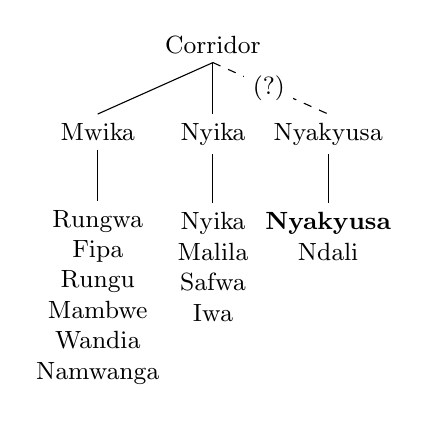
\begin{tikzpicture}[level distance=2.5em,
			sibling distance=8em,
			parent anchor=south,
			child anchor=north,
			anchor=north,
			align=center]
\small
\node(A){Corridor}
	child[sibling distance=4.5em]
			{node {Mwika} edge from parent[solid]
				child[sibling distance=4.5em]	
					%%M26 Iwa zweimal? Am Buch checken!		
					{node {Rungwa\\Fipa\\Rungu\\Mambwe\\Wandia\\Namwanga} edge from parent[solid]}
			}
	child[sibling distance=4.5em]
			{node {Nyika} edge from parent[solid]
				child[sibling distance=4.5em]
					{node {Nyika\\Malila\\Safwa\\Iwa} edge from parent[solid]}	
			}
	child[sibling distance=4.5em]
			{node (B){Nyakyusa} edge from parent[dashed]
				child[sibling distance=4.5em]
					{node {\textbf{Nyakyusa}\\Ndali} edge from parent[solid]}
			}	
;	
\path (A) -- coordinate[midway](AB) (B);
\node [anchor=center,fill=white] at (AB) {(?)};
\end{tikzpicture}
\caption{Nurse \& Philipson's (\citeyear{NurseDPhillipsonG2003b}) classification of the Corridor languages}\label{ClassificationNursePhillipson2003}\il{Rungwa}\il{Fipa}\il{Rungu}\il{Mambwe}\il{Wandia}\il{Namwanga}\il{Nyika}\il{Malila}\il{Safwa}\il{Iwa}\il{Ndali}
\end{center}
\end{figure} 
Catherine Labroussi's (\citeyear{LabroussiC1998}, \citeyear{LabroussiC1999}) work is a valuable contribution to our understanding of the Corridor languages: apart from phonological traits and lexicostatistic calculations, it examines patterns of diffusion and also discusses social factors, mostly retrieved by archaeology and oral history. As for the classification of the Corridor languages, it fundamentally reflects Nurse's position concerning Nyakyusa.

Historian Christopher Ehret (\citeyear{EhretC1973}) proposed a Corridor-group (``Mambwe-Fi\-pa-Nyiha'')\il{Mambwe}\il{Fipa}\il{Nyika} which excludes Nyakyusa. What distinguishes his proposal is that he postulates that Corridor and Nyakyusa may belong to different branches of eastern Bantu. This position is revised in \citet[36f, 55]{EhretC2001}, where the Corridor languages are split into two major groups, Rungwe (Nyakyusa, Ndali,\il{Ndali} Safwa,\il{Safwa} Nyika,\il{Nyika} Wandia\il{Wandia}) and Mwika (Pimbwe,\il{Pimbwe} Fipa,\il{Fipa} Mambwe,\il{Mambwe} Namwanga\il{Namwanga}). Ehret qualifies this insofar as he admits that this synchronic grouping need not reflect linguistic genealogy.

Ehret's student Catherine Fourshey, however, has returned to Ehret's earlier views \citep{FoursheyC2002}. In an attempt to reconstruct the pre-colonial history of the Corridor based mainly on linguistic data, she proposes a genetic unit comprising the Corridor languages, with the internal structure of this unit in essence reflecting Nurse's classification. Fourshey arrives at this assumption primarily on the basis of lexicostatistics supplemented and refined by an examination of the distribution of certain cultural lexemes. Unfortunately Fourshey did not have access to the linguistically more fine-grained analysis of \citet{LabroussiC1998}.

To conclude, it seems safe to assert at this point -- as stated more or less explicitly in \citet{NurseD1988}, \citet{LabroussiC1998}, \citet{NurseDPhillipsonG2003b} -- that the languages of the Corridor might best be understood not as a genetically uniform unit, but as forming an area of long-term linguistic convergence. In this context, Nyakyusa can be understood as the special case, being more strongly isolated from its geolinguistic environment. Although it shares a number of lexical and structural features with its neighbouring languages, especially \ili{Ngonde} and \ili{Ndali}/Sukwa,\il{Sukwa} it seems to have been rather resistant to external influences, and in the development and spreading of innovations it seems to have played the role of donor rather than that of recipient.

\largerpage[-2]
\subsection{Dialects and variety described}\label{InternalClassiffication}
\is{dialects|(}
The dialectal geography of the Corridor as a whole, as well as for the specific case of Nyakyusa, remains relatively unknown (\citealt[4, 25]{WalshMSwillaI2002}). However, a number of topolectal divisions can be stated. Some first observations concerning subgroups and varieties of Nyakyusa were made by \citet[61]{JohnstonH1977}, with subsequent refinements by \citet[2]{WilsonM1963}. The following notes are based on the latter, as well as on \citeauthor{WalshMSwillaI2002}'s (\citeyear{WalshMSwillaI2002}) comments upon it. These sources have been supplemented by consultation with a number of native speaker informants as well as by an unpublished survey by SIL International.\footnote{Kindly made available to the author by Helen Eaton.\ia{Eaton, Helen}} The following list gives the identifiable subgroups within Nyakyusa, together with their respective Guthrie codes according to \citet{MahoJ2009}:\footnote{It has to be kept in mind that ethnic or group identity and linguistic varieties need not overlap.}
\begin{compactitem}
\item Nyakyusa of the lake-shore plains. This variety is often referred to as \textit{MuNgonde} by speakers of northern varieties, although speakers from the area do not use this name themselves. It is considered clearly distinct from Malawian \ili{Ngonde} (\mbox{\textit{IkyaNgonde}}).
\item Central Nyakyusa, around Masoko. The Nyakyusa variety of this area, seat of chief Mwaipopo, is considered the variety with the highest prestige. In \citet{MahoJ2009} this variety is grouped with that of the lake-shore plains as \textit{Nyakyusa proper} (M31A).
\item Northern Nyakyusa (M31B), also called \textit{Kukwe} or \textit{Ngumba} (`innermost plateau').
\item Nyakyusa of the mountains (M31C), also referred to as \textit{Mwamba} (`Mountains'), \textit{Lugulu} (name of an aboriginal group) or \textit{Sokelo} (`East'), in the area around Mwakaleli.
\item Selya (M31E), at the foot of the Livingstone Mountains. Wilson distinguishes this from another eastern subgroup named Saku.
\end{compactitem}
The denominations for the various groups and varieties within Nyakyusa are used differently by speakers from different areas. As Monica Wilson states:
\begin{quote}AbaMwamba means by derivation `the hill people', but is generally used for `the people of the north'. The \ili{Ngonde} of Karonga call those on the plain around Mwaya BaMwamba, the men of Mwaya apply the name not to themselves, but to the people of Selya, while the people of Selya apply it to those in the hills to the north of them. \citep[2 FN2]{WilsonM1963}
\end{quote}
\largerpage[-2]
Two further varieties of unclear status might be added to the list above. \citet[9]{WilsonM1958} observed that the group of \ili{Penja} M302, as well speakers of the eastern variety of \ili{Nyika} M23, were being absorbed by the Nyakyusa. While the case of \ili{Penja} remains unsolved \citep[26]{WalshMSwillaI2002}, a recent sociolinguistic survey provides further indications of a language shift of the Eastern \ili{Nyika} people, suggesting an additional Nyakyusa topolect \citep{Lindforsetal2009}. 

Although diatopic variation within Nyakyusa exists and speakers readily identify the speech varieties of different regions, intercomprehension is not affected. Given the high number of speakers, Nyakyusa can be considered relatively uniform in comparison to many of the other, smaller Corridor languages (see \citealt[204]{LabroussiC1998}). Most speakers consulted stress that the main dividing line lies between the variety of the lake-shore plains (Kyela district) on the one side and the varieties of the more mountainous terrains on the other.

The focus of this study lies on the Selya and Mwamba/Lugulu varieties. The Germany-based language assistants are originaly from Ikama (Mwamba/Lugulu) and Itete (Selya). In Mbeya city, preliminary work was performed with speakers from Itete. The main part of the fieldwork (\sectref{DataCollection}) took place in the village of Lwangwa, which is said to be at the transition between the Mwamba/Lugulu and Selya varieties. The map in \figref{MapLwangwaIkamaItete} shows the position of the three villages.

\begin{figure}[hbt]
\begin{center}
\includegraphics[width=0.75\textwidth]{figures/MapLwangwaIkamaItete.png}
\caption{Field base and origin of language assistants. Map courtesy of Monika Feinen}
\label{MapLwangwaIkamaItete}
\end{center}
\end{figure}

\label{Varietydescribed}
 \is{dialects|)}
\section{Data collection}\label{DataCollection}
The main data for this study was collected during three research trips to Tanzania. The first trip took place in November and December 2013, during which time research was carried out with speakers living in the city of Mbeya. On the second trip, in November and December of 2014, as well as on the third trip, from late September to early December of 2015, Lwangwa village in Busekelo district was chosen as the field base. Further intensive work, mainly guided elicitation, was carried out with two language assistants living in Germany between 2012 and 2016.

All language assistants that participated in this study are native speakers of Nyakyusa, fluent in Swahili and between 25 years and 78 years of age during the period of research. The expatriate speakers have been living in Germany since 2009 and 2005 respectively. Since that time they have returned periodically to the language area and continue to converse with family members on a regular basis in their native language. The contact language used in research has mainly been English, plus some Swahili (in Tanzania) and German (in Germany). 

The main practices of data collection were one-on-one elicitation and text collection, predominantly of folk narratives. Elicitation is here to be understood not as a mere production task, but in a broad and interactive sense, in line with \citet[2]{MousM2007}, who states that ``elicitation is guided conversation about language data''. See \citet[245--256]{CoverR2015} for a recent discussion of elicitation with a focus on semantic fieldwork.

The collection of lexical items, apart from basic approaches such as the elicitation of semantic fields and sound-substitution \citep[104--111]{CrowleyT2007}, was greatly aided by previous work on Nyakyusa, especially \citeauthor{FelbergK1996}'s (\citeyear{FelbergK1996}) dictionary. Although a great number of entries had to be checked for accuracy, it served as a valuable starting point for enlarging the lexical corpus. All lexical items were entered into a database using Fieldworks Language Explorer (FLEx) software. In the course of research this was supplemented and double-checked with usage in texts and spontaneous speech. FLEx software was also used for morphological segmentation and creating lexical cross-references. Given the problematic representation of Nyakyusa in several recent publications (see \sectref{ResearchHistory}), 
a great amount of time and scrutiny was dedicated to checking and re-checking all transcriptions.

With regard to the semantics of TMA, elicitation encompassed a variety of tasks. One of them was translation from the contact language, mostly together with a discourse context. Here \citeauthor{DahlOe1985}'s (\citeyear{DahlOe1985}; \citeyear{DahlOe2000a}) tense and aspect questionnaires served as valuable points of departure. In other cases, the compatibility of a given construction with specific adverbials or lexical items was checked through grammaticality judgements, or possible contexts of use for constructed sentences were narrowed down through dialogue with the language assistants. The more research advanced, the more elicitation on TMA became intertwined with the analysis of texts and naturally observed data. Specific utterances were checked for their applicability and/or meaning in other contexts, and examples were manipulated in a targeted way, again checking for acceptability, changes in meaning, and possible contexts of use.

The texts used in this study came from two main sources. First, oral monologues, mostly folk narratives plus a few \isi{expository} texts, were recorded with single speakers and later transcribed by the researcher. The transcription was then checked and the texts were translated into English with the help of a language assistant. Apart from minor exceptions, these were not the recorded speakers themselves. Additionally, two retellings of the Pear Story \citep{ChafeW1980} were recorded and one oral rendering of a traditional narrative was made available by Knut Felberg.
Furthermore, a number of written texts were made available by SIL International's Mbeya office. These stem from literacy workshops and are mostly fictitious narratives but also include a few \isi{expository} and \isi{procedural} texts and one \isi{behavioural} text. Five of these came edited and with translations into English, the others were translated with the language assistants. One additional written expository text was provided by one of the main language assistants. All written texts were double-checked for pronunciation. The composition of the text corpus is given in \tabref{CompositionTextCorpus}. A few additional examples were taken from a current draft of a Bible translation by SIL International (kindly made available by Helen Eaton\ia{Eaton, Helen}),\footnote{Scripture quotations from The Authorized (King James) Version. Rights in the Authorized Version in the United Kingdom are vested in the Crown. Reproduced by permission of the Crown’s patentee, Cambridge University Press.} HIV prevention materials produced by the same organization and older text collections (\citealt{BergerP1933}; \citealt{BusseJ1942}; \citeyear{BusseJ1949}).


\begin{table}[ht]
\begin{center}
\begin{tabular}{lllll}

\lsptoprule

\footnotesize{Genre} & \footnotesize{Medium} & \footnotesize{Source} & \footnotesize{N\textsuperscript{o}\xspace of texts} & \footnotesize{Avg. N\textsuperscript{o}\xspace of words}\\
\midrule

Narrative & Oral & Own fieldwork & 15 & 324\\
Narrative & Oral & Knut Felberg & 1 & 856\\
Narrative & Written & SIL & 16 & 285\\
Retelling & Oral & Own fieldwork & 2 & 430\\
Exposition & Oral & Own fieldwork & 3 & 351\\
Exposition & Written & Own fieldwork & 1 & 95\\
Exposition & Written & SIL & 2 & 247\\
Behavioural & Written & SIL & 1 & 129\\
Procedural & Written & SIL & 1 & 205\\
\lspbottomrule
\end{tabular}
\caption{Composition of the text corpus}
\label{CompositionTextCorpus}
\end{center}
\end{table}
\largerpage[1]
The focus on \isi{narrative} discourse is due to a number of reasons. The first reason is the availability of texts and the comparatively easy segmentation of narrative texts, given the time limits imposed upon this study. The second reason is the need for an adequate description of the dedicated narrative markers (Chapter \ref{NarrativeMarkers}). Third, though monological in their form, narratives often contain language of other communicative situations, for instance episodes in dialogue form or embedded expository or behavioural discourse. The use of certain grammatical devices, especially TMA, in everyday discourse constitutes an area that is open for further research.

Apart from elicitation and text collection, a great deal of everyday life in the field was carried out using Nyakyusa. This allowed for the observation of language use in a more natural environment and proved a fruitful source for contextualized examples, which served as jumping-off points for further elicitation. Lastly, \ili{Proto-Bantu} reconstructions stem from the Bantu lexical reconstructions\nobreakspace 3 database \citep{BLR3}.

Throughout this study, examples from elicitation sessions are marked with the abbreviation \lq\lq[ET]''. Textual data is marked with a short version of the text's name, often the title of the narrative, such as \lq\lq[Crocodile and Monkey]''. Examples from participant observation or conversation are marked as \lq\lq[overheard]''.
\section{Theoretical framework}\label{TheoreticalFramework}
\subsection{Overview}
For most parts of this grammar, no particular framework has been adopted. Instead, the description is based on well-known descriptive and typological concepts. In those parts dealing with phonological, morphological and syntactic aspects, the description is guided by structural considerations, whereas in the discussion of the meaning and use of TMA categories, functional considerations are in the foreground.

However, to gain a more profound understanding of the organization of \isi{tense} and aspect,\is{aspect!grammatical} the cognitive framework developed by \citet{BotneRKershnerT2008} has been adopted, although an attempt was made to give a broad and dense description so as to facilitate translation into other frameworks. Botne \& Kershner's framework will be outlined in \sectref{TenseAspect}--\ref{InherentTemporalStructure}.
 
Further, to approach the uses of TMA categories in Nyakyusa \isi{narrative} texts, the analytic tools developed by \citeauthor{LabovWWaletzkyJ1967} (\citeyear{LabovWWaletzkyJ1967} and subsequent works) were applied and augmented by a number of concepts stemming from the works of Fleischman (esp. \citeyear{FleischmanS1990}) and \citeauthor{LongacreR1990} (esp. \citeyear{LongacreR1990}), as well as by some insights into activation status by Prince (\citeyear{PrinceEF1981}; \citeyear{PrinceEF1992}). All these are described in \sectref{ToolsNarrativeAnalysis}. Lastly, while the approaches mentioned so far are synchronically oriented, in various cases it was found that applying a diachronic perspective helped the understanding of the present-day situation. Therefore, findings from \isi{grammaticalization} theory (e.g. \citealt{HeineBClaudiUHuennemeyerF1991}; \citealt{BybeePerkinsPaglucia1994}) were included, particularly with regard to identifying the sources of a given construction, delimiting newer and older readings and disentangling the interplay between the various constructions available within an area of grammar.
\subsection{Tense and grammatical aspect}\label{TenseAspect}
\subsubsection{Tense}\label{Tense}
\is{tense|(}
Tense is a deictic category that localizes a described state-of-affairs in time (see \citealt{ComrieB1985} among others). According to the most commonly expressed view, the linguistic construal of time is best described in terms of an abstract time line. Thus \citet[2]{ComrieB1985}, in his reference work on tense, declares that \lq\lq such a diagrammatic representation of time is adequate for an account of tense in human language.” \figref{FigureLinearConceptionOfTime} illustrates this conception. Throughout this study, in the illustration of temporal relations, S stands for \lq time of speech’.

\begin{figure}[h]
\begin{center}
\includegraphics{figures/GrafikLinearTime.eps}
\caption{Linear conception of time}
\label{FigureLinearConceptionOfTime}
\end{center}
\end{figure}

Bantu languages are well known for their complex TMA systems which include various degrees of remoteness in time, especially in the past (\citealt[185]{DahlOe1985}; \citealt[21f]{NurseD2008}). Following the common conception of tense, these are usually described in terms of distance on a mono-dimensional timeline, as illustrated in \figref{FigureRemoteness}. The subscript digits indicate the degree of remoteness.

\begin{figure}[h]
\begin{center}
\includegraphics{figures/GrafikRemoteness.eps}
\caption{Remoteness distinctions in a linear conception of time}
\label{FigureRemoteness}
\end{center}
\end{figure}

Such a representation, however, fails in many cases to explain patterns of morphological marking, as well as the systematic employment of these constructions. For example, the Malawian Bantu language \ili{Sukwa} M301, as discussed by \citet[93f]{KershnerT2002}, possesses four non-imperfective paradigms with past time reference. At first glance, their meanings seem to represent a progression from immediate past to to remote past. \figref{FigureSukwaPasts} illustrates these paradigms together with their morphological composition on the traditional timeline.

\begin{figure}[hbt]
\begin{center}
\includegraphics{figures/GrafikPastsSukwa.eps}
\caption{Sukwa paradigms with past reference. Adapted from \citet[94]{KershnerT2002}}
\label{FigureSukwaPasts}
\end{center}
\end{figure}

The linear approach to tense fails to give a motivated explanation for the morphological composition of these constructions, e.g. why there is a zero-prefix in past\textsubscript{2}, whereas past\textsubscript{1} and past\textsubscript{3} have \textit{aa}-, or why past\textsubscript{3} combines the prefix of past\textsubscript{1} with the suffix of past\textsubscript{2}. Further, it does not allow us to adequately describe their patterns of employment, which are described at length by \citet{KershnerT2002}.

To address such cases, \citet{BotneRKershnerT2008} develop a cognitive model of tense and aspect, which is based on the tenet that there are two basic conceptualizations of time. One conceptualization has Ego, the conceptualizer, moving along a stationary timeline (\textsc{time is a path}); see \citet[84f]{EvansVGreenM2006} on the concept of Ego. In the other, time itself is construed as moving (\textsc{time is a stream}), which allows for two perspectives. Either the metaphorical stream of time moves Ego along, passing eventualities as they take place, or time floats eventualities past a stationary Ego. \figref{FigurePerspectivesOnTime} depicts the two basic construals.

\begin{figure}[h]
\begin{center}
\includegraphics{figures/GrafikPerspectivesTime.eps}
\caption{Two perspectives on time}
\label{FigurePerspectivesOnTime}
\end{center}
\end{figure}

These two distinct conceptualizations of time are not mutually exclusive. A language may rather encode different aspects of both in different verbal paradigms. Botne \& Kershner go on to decompose \citeauthor{ReichenbachH1947}'s (\citeyear{ReichenbachH1947}) concept of reference time into two separate concepts: reference frame (\lq\lq temporal domain'' in Botne \& Kershner's terms) and reference anchor. The first is said to be \lq\lq comparable, but not identical'' \citep[152]{BotneRKershnerT2008} to \citeauthor{KleinW1994}'s (\citeyear{KleinW1994}) concept of topic time. Tense is then understood as the relationship between time of speech as the deictic locus and a reference frame. When the time span of the reference frame includes the deictic locus, this ``denot[es] a primary, prevailing experiential past and future perspective'' \citep[153]{BotneRKershnerT2008}. In cases where the deictic locus is not included in the time span of the reference frame (domain), they speak of a dissociated past or future. Exclusion corresponds to the conceptualization of \textsc{time} is a \textsc{path}.

The split between reference frame and reference anchor allows Botne \& Kershner to further account for temporal relations within a reference frame, which correspond to the conceptualizatioan of \textsc{time} is a \textsc{stream}. 

\figref{PastDDomain} illustrates these two types of temporal relationships, with the reference frames (domains) as rectangular plains. \figref{PastDDomain}a depicts a past tense, such as the \ili{English} simple past. With the reference frame excluding the time of speech, the conceptualizer is instructed to move to a different cognitive domain, where the eventuality takes place. \figref{PastDDomain}b illustrates an associated past (\lq\lq tenor'' in Botne \& Kershner's terminology), which situates an eventuality prior to the time of speech but within the same reference frame.

\begin{figure}[th]
\caption{\label{PastDDomain}Dissociative and associative pasts}
\subfigure[Dissociative past]{
\includegraphics[width=0.45\textwidth]{figures/GrafikPastDDomainNew.eps}
}
\subfigure[Associative past]{
\includegraphics[width=0.45\textwidth]{figures/GrafikPastPDomainNew.eps}
}
\end{figure}

\largerpage
In the case of \ili{Sukwa} addressed above, constructions with past time reference can now be described on a compositional basis \citep{KershnerT2002}. The suffix \mbox{-\textit{ite}} denotes \textit{completive aspect}.\footnote{See \sectref{Aspect}, \ref{PerfectivityCompletion} on grammatical aspect\is{aspect!grammatical} and the notion of \isi{completion}, respectively.} The prefix \textit{aa}- situates the described state-of-affairs in a preceding time unit within the same reference frame. In out-of-the-blue utterances this is understood as being shortly before the time of speech, but depending on the discursive environment, it can also refer to units such as the preceding day, month, season, etc.
The sense of heightened remoteness of the configuration \mbox{\textit{aa}-}\textsc{vb}\mbox{-\textit{ite}} then derives from viewing an event as already completed within a preceding time unit. Lastly, \textit{ka}- is a true tense in that it situates the state-of-affairs in a past reference frame. \figref{FigureSukwaTenorTense} illustrates the pasts of Sukwa.\il{Sukwa} See \citet{BotneRKershnerT2008} for a discussion of a number of such cases across Bantu.

\begin{figure}[tbh]
\caption{\label{FigureSukwaTenorTense}Organization of the past in Sukwa. Adapted from \citet[113]{KershnerT2002}.}
\begin{center}
\includegraphics{figures/GrafikSukwaTenorTenseNew.eps}
\end{center}
\end{figure}

Apart from Botne \& Kershner's own work (among others \citealt{BotneR2003b}; \citeyear{BotneR2006}; \citeyear{BotneR2008}; \citealt{BotneRKershnerT2000}; \citeyear{BotneRKershnerT2008}; \citealt{KershnerT2002}) their framework has proven fruitful in \citeauthor{SeidelF2008}'s (\citeyear{SeidelF2008}) grammar of \ili{Yeyi} R41, \citeauthor{CraneTM2011}'s (\citeyear{CraneTM2011}) treatise of tense and aspect in \ili{Totela} K41 as well as \citeauthor{DomSBostoenK2015}'s (\citeyear{DomSBostoenK2015}) work on the \ili{Kikongo} cluster of Bantu languages. As will be seen in Chapters \ref{TenseAspectConstructions}--\ref{Futurates}, the core assumption of two linguistic perspectives on time will also guide our understanding of the organization of the Nyakyusa tense and aspect system.
\is{tense|)}

 
\subsubsection{Grammatical aspect}\label{Aspect}
\is{aspect!grammatical|(}
While tense, as defined in \sectref{Tense}, is a deictic category, aspect is not. According to the most common and widely agreed-upon definition, ``aspects are different ways of viewing the internal temporal constituency of a situation'' \mbox{\citep[3]{ComrieB1976}.}

\newpage 
As has been pointed out variously in the theoretical literature on aspectuality, it is essential to distinguish aspect as a grammatical device from the aspectual potential encoded in the lexical verb or verb phrase. \citet{SasseHJ2002} speaks of \lq\lq bidimensional approaches'' to aspectuality. Within these bidimensional approaches, a prominent position is taken by those approaches which \citet{SasseHJ2002}, adopting a term first introduced by \citet{BickelB1997}, calls \lq\lq radical selection theories''. In these theories, aspect as a morphosyntactic device and the lexical dimension of aspect are understood as standing in a strict correspondence relationship: grammatical aspect serves as a phase-selector that selects matching temporal phases from the lexical dimension (the concept of phase will be developed in \sectref{InherentTemporalStructure}). As Sasse points out, other prominent bidimensional approaches to aspectuality, such as the one put forward by \citet{SmithC1997}, are conceptually closely related to radical selection theories or might even constitute only a notional variant of them.

The need to distinguish two dimensions of aspectuality also holds for an adequate description of Nyakyusa. As will become clear in Chapters \ref{AspectualClassification}--\ref{Futurates}, grammatical aspect in Nyakyusa is sensitive to the aspectual potential in the lexical (and verb phrase) dimension and hence the choice of an inflectional paradigm greatly depends upon the latter. A central distinction here is that which falls between inchoative and non-inchoative verbs; see \sectref{AristotelianAspect}. In compliance with the tenets of radical selection theories, Botne \& Kershner define grammatical aspect as follows:

\begin{quote}
[Grammatical, BP] [a]spect denotes the particular temporal view of time in the narrated event. More precisely, a specific aspect denotes a particular temporal phase of the narrated event as the focal frame for viewing the event. This focal frame depicts the status of the event in relation to the vantage point determined by Ego, by default typically the moment of speaking. \citep[171]{BotneRKershnerT2008}
\end{quote}

It is not entirely clear how far the idea of a temporal phase as the ``focal frame'' serves our understanding of grammatical aspect in Nyakyusa. Rather, it seems, especially in the case of perfective aspect (\sectref{PerfectivityCompletion}), that Ego's vantage point may be construed in relation to a particular phase without necessarily being contained in the eventuality itself. Throughout this study, grammatical aspect will therefore be understood in a slightly simplified version of Botne \& Kershner's definition as denoting a particular temporal view of an eventuality by relating Ego's vantage point to a particular temporal phase of it.

As can be gathered from the preceding discussion, Botne \& Kershner's approach to tense and grammatical aspect is a compositional one. Concerning Nyakyusa, this has proven especially fruitful for the analysis of the past tense paradigms (see Chapter \ref{TenseAspectConstructions}), the function of the future enclitic \textit{aa}= (\sectref{ProcliticAa}) and the analysis of the present perfective (\sectref{PresentPerfective}) vis-à-vis the past perfective (\sectref{PastPerfective}). In a few other cases, such as the narrative tense (\sectref{NarrativeTense}) and the modal future (\sectref{ModalFuture}), the meanings and uses of the paradigms in question can, however, only be taken as a function of the entire construction. This situation can, in turn, be explained by taking into account the diachronic axis.
\is{aspect!grammatical|)}
\subsection{Inherent temporal structure of the verb}\label{InherentTemporalStructure}
Grammatical aspect,\is{aspect!grammatical} as defined in the previous subsection, relates Ego's vantage point to a particular temporal \isi{phase} of an eventuality. The key to the interpretation of any particular verbal expression in Nyakyusa is thus the interaction between grammatical aspect\is{aspect!grammatical} and the temporal structure inherently encoded in the verb. In spite of its central role, this facet of grammar hardly receives any attention in descriptive work on Bantu languages. It is common in Bantu studies, however, to recognize that a number of verbs tend to show a particular behaviour, appearing mainly in certain inflectional paradigms and encoding a state. This class of verbs is commonly labeled \lq\lq inchoative verbs'' (e.g. \citealt[55–60]{ColeD1955});\is{inchoative verbs} this class of verbs will be dealt with in more detail below. A brief theoretical digression will lay out the concepts and analytical tools central to understanding the interaction between the lexical and the inflectional dimension in Nyakyusa.
\subsubsection{Aristotelian aspect (\lq lexical aspect')}\label{AristotelianAspect}
\is{aspect!Aristotelian|(}Aristotelian aspect, also named \lq lexical aspect' or \lq verb aspect' by some scholars, refers to the obligatory classification of the aspectual potential encoded in the lexical (and phrasal) dimension in terms of abstract temporal phases. \citet{SasseHJ2002} speaks of \lq aspect\textsubscript{2}'. The present study follows Binnick's terminology, as \iai{Aristotle} is generally credited with discovering these distinctions \citep[171f]{BinnickR1991}.

The most familiar categorization of verbal expressions in the linguistic literature are the categories postulated by the philosopher \citet{VendlerZ1957} and developed to explain the behaviour of different verbal expressions in English.\il{English} Vendler\ia{Vendler, Zeno} distinguishes four types of expressions based on temporal criteria and their behaviour or compatibility in particular syntactic frames: states, activities, achievements and accomplishments. A major split between these categories is along the lines of telicity (delimitedness): achievements and accomplishments are understood as telic, whereas states and activities are understood as atelic. The latter two again differ in dynamicity, while accomplishments and achievements differ in regards to their duration (see below). Vendler's\ia{Vendler, Zeno} categories have been accepted by a great number of scholars as being valid for all natural languages, as they are supposed to be based on universals of logic and are therefore understood not to be subject to cross-linguistic variation (see e.g. \citealt[322]{TatevosovS2002}); for critical evaluations of this assumption see \citet{FilipH2011} and \citet{Bar-elL2015}. The broad acceptance of Vendler's\ia{Vendler, Zeno} categorization is not challenged by certain tweaks proposed by different scholars: for instance \citet{VerkuylH1972} and \citet{KennyA1969} conflate achievements and accomplishments, while \citet{SmithC1997} adds semelfactives as a further category. A number of tests to determine the category of different expressions have been developed in the literature, the most cited test being one for telicity, by checking for compatibility with adverbials of the type ``in X time'' and ``for X time''. For an overview of tests put forward by a number of scholars, see \citet[173–197]{BinnickR1991}.

For the study of Bantu languages Vendler's\ia{Vendler, Zeno} categories are hardly applicable. As \citeauthor{CraneTM2011} puts it:
\begin{quote}Rather than having a basic telic-atelic distinction, Bantu languages in general appear to divide verbs differently. This is due to a distinction between non-inchoative verbs (roughly corresponding to Vendler’s states, activities, and accomplishments) and inchoative verbs, which encompass many of Vendler’s\ia{Vendler, Zeno} achievements and other verbs. \citep[34]{CraneTM2011}\end{quote}

Crane hints at two closely related points of central importance. First, one essentially problematic category in Vendler's classification is that of achievement verbs. In a Vendlerian\ia{Vendler, Zeno} understanding, as echoed by \citet[195]{BinnickR1991}, ``an achievement is all culmination; although the achievement is possibly preceded by some activity […] the verb refers only to the achievement phase, not to the preceding activity''. \citet{PersohnB2017b}, by drawing on the Nyakyusa data presented in Chapter \ref{AspectualClassification} and incorporating data from \ili{Sukwa} \citep{KershnerT2002} and \ili{Ndali} \citep{BotneR2008}, shows that the morphosemantic behaviour of numerous verbal lexemes and verb phrases in these languages can only be explained by assuming the lexicalization of transitional patterns that consist of a state or process of origin, a change-of-state and a resultant state; similar assumptions have so far been mostly implicit in recent studies of aspectuality in Bantu languages. This leads to the second point: Crane picks up the notion of \textit{inchoative verbs},\is{inchoative verbs} which has come to be used as an umbrella term for those classes of verbal lexemes that encode a resultant state as part of their aspectual potential. As will become more explicit in Chapters \ref{AspectualClassification}--\ref{TenseAspectConstructions}, this notion of inchoativity plays a central role in the choice of grammatical aspect in Nyakyusa.

Within radical selection theories of aspectuality (\sectref{Aspect}), certain modifications of the Vendlerian\ia{Vendler, Zeno} categories have been stipulated. To give an example, Breu and Sasse (e.g. \citealt{BreuW1984}; \citealt{SasseHJ1991}) understand grammatical aspect\is{aspect!grammatical} as making reference to boundaries of situations, the basic assumption being that the lexical or verb phrase dimension can potentially encode one situation, a left boundary that represents the ingression into the situation and a right boundary, that is, the egression out of the situation. This yields five potential types of verbs. Other radical selection theories, such as \citet{BickelB1997} or \citeauthor{JohansonL1996} (\citeyear{JohansonL1996}; \citeyear{JohansonL2000}) offer comparable classifications; see \citet[48–52]{CroftW2012} for an overview. What these approaches share is the basic assumption that the lexical or verb phrase dimension may encode only one situation (or \lq middle phase'), which by definition excludes any lexicalizations of a transition from a state or process of origin into a resultant state; see \citet{PersohnB2017b} for more extensive discussion.

For the description of aspectuality in Nyakyusa the present study thus draws on a framework developed by Botne and Kershner (see \citealt{BotneR1983}; \citealt{KershnerT2002}; \citealt{BotneRKershnerT2008} among others; see also \sectref{TenseAspect}), which has its origin in Botne's study of aspectuality in Ruanda JD61 and which has been extended by Kershner's study of Sukwa M301.\il{Sukwa} Botne and Kershner's categorization of verbs is based on \citet{FreedA1979}, a study of \ili{English} \isi{phasal verbs} (\lq aspectualizers') and their interaction with verbal semantics and the syntax of the verbal complement, in which Freed provides a formalization of Vendler's\ia{Vendler, Zeno} categories. In analogy with syllable phonology Freed\ia{Freed, Alice} proposes that the underlying temporal structure of verbs can be understood as a combination of three phases\is{phase} (\lq\lq segments'' in her terminology). The Onset\is{phase!Onset phase} constitutes a preliminary or preparatory phase, while the Nucleus\is{phase!Nucleus phase} corresponds to the characteristic act encoded in the verb. The Coda\is{phase!Coda phase} constitutes a culminative phase following the characteristic act. In doing so, Freed\ia{Freed, Alice} subscribes to Vendler's\ia{Vendler, Zeno} understanding of achievements as pure transitions. Botne and Kershner, in their works, adopt Freed's\ia{Freed, Alice} understanding of phases;\is{phase} their central modification is to allow for more combinations of phases.\is{phase} Thus achievement verbs, apart from a punctual Nucleus,\is{phase!Nucleus phase} may further encode an extended Onset\is{phase!Onset phase} (state of origin) and/or an extended Coda\is{phase!Coda phase} (resultant state), yielding four types of achievements. Likewise, accomplishments may either contain a punctual or extended Coda\is{phase!Coda phase} phase. In both cases, the presence or absence of an extended Coda phase\is{phase!Coda phase} is equivalent to the distinction between inchoative\is{inchoative verbs} and non-inchoative verbs. Activities, in Botne \& Kershner's understanding, comprise an extended Nucleus,\is{phase!Nucleus phase} whereas a state does not possess any internal structure. Throughout this study, in illustrations of aspectual classes the three possible constituent phases\is{phase} will be abbreviated as O, N and C, respectively. Note that the choice of Botne \& Kershner's model is to be understood as a useful descriptive tool; see \citet{PersohnB2017b} for a critical evaluation.   

What must be emphasized in this context is the essential need to distinguish between the ontology of a real world state-of-affairs on the one hand and the linguistic construction (lexicalization) on the other, which need not be congruent (\citealt[77–100]{BotneR1981}; \citealt{BickelB1997}). Stated differently, cross-linguistic differences can arise when different phases\is{phase} of a situation are included in the lexical semantics of a verb. This is illustrated by \citet{BotneR2003b}, a case study on \lq to die' verbs, traditionally understood as a primary example of an achievement in Vendler's\ia{Vendler, Zeno} sense. Furthermore, the alleged polysemy of many inchoative verbs\is{inchoative verbs} in Bantu (\lq to become X'; \lq to be X') can thus be understood as a result of an inadequate meta-language translation, rather than an as inherent ambiguity (cf. \citealt[269, FN 249]{SeidelF2008}).
\subsubsection{Aktionsart}\label{Aktionsart}
\is{aktionsart|(}Having broached the issues of grammatical aspect\is{aspect!grammatical} and Aristotelian (lexical) aspect,\is{aspect!Aristotelian} a further analytical distinction is to be made between Aristotelian aspect and Aktionsart. While Aristotelian aspect classifies the phasal structure of the verb in a wider sense, Aktionsart is ``rather a classification of (expressions for) phases of situations and subsituations'' (\citealt[170]{BinnickR1991}), which is optional and best described in more specific terms such as inceptive or resumptive \citep[ibid]{BinnickR1991}. Formally, Aktionsart in Nyakyusa is expressed by verbal derivation (Chapter \ref{VerbalDerivation}) and \isi{phasal verbs} (Chapter \ref{AspectualClassification}).

To give an example, in the single-event reading of (\ref{exAktionsart}) the phasal verb\is{phasal verbs} \textit{leka} \lq cease, stop' refers to a cessation of the Nucleus phase of the lexical verb \textit{moga} \lq dance':

\begin{exe}
	\ex\label{exAktionsart}
	 \gll a-lek-ile ʊ-kʊ-mog-a\\
	1-cease-\textsc{pfv} \textsc{aug}-15(\textsc{inf})-dance-\textsc{fv}\\
	\glt \lq S/he has stopped dancing.'
\end{exe}
\is{aktionsart|)}
\subsection{Tense and grammatical aspect in discourse}\label{TenseAspectDiscourse}
\subsubsection{Remarks on textual analysis and grammaticography}
In the following description of tense and aspect categories, apart from their use in a sentence-level frame, an attempt is made to further include their use in discourse. A number of factors speak in favour of this approach. The \lq traditional' perspective on tense and aspect is most clearly expressed by Comrie:
\begin{quote}{[T]he investigation of the use of a grammatical category in discourse should not be confused with the meaning of that category; instead, the discourse function should ultimately be accounted for in terms of the interaction of meaning and context. \citep[29]{ComrieB1985}}\end{quote}

Among the well-known feature of Bantu languages, however, are constructions whose main function lies in the structuring of narrative discourse \citep[24]{NurseD2008}, typically labelled \textit{narrative tense} and/or \textit{consecutive tense}; see Chapter \ref{NarrativeMarkers} for such constructions in Nyakyusa.\is{narrative markers} Thus Comrie's perspective seems problematic with regard to descriptive adequacy. A similar argument is put forward by \citet{GueldemannT1996} in his discussion of Doke's grammar of \ili{Lamba} M54 (translated from the original German, BP):
\begin{quote}{In the otherwise extensive and precise grammatical analysis by Doke one hardly encounters useful indications concerning the construction's functional classification […] The author only describes the verbal paradigm with\-in the limits of sentence semantics […] Within such an approach the result of the analysis can only produce a relatively vague term such as tempus historicum, which semantically speaking seems the more vacuous as the paradigms characterized by it are not the only ones that can denote historical events. \citep[208]{GueldemannT1996}}\end{quote}

Furthermore, as \citet[77--79]{LevinsonS1983} notes, in most languages there is no one-to-one correspondence between temporal reference, in the physical sense, and linguistic categories. It is a common feature of natural languages to employ the latter for a broader variety of meanings. Assuming these notions surface especially in discourse contexts, an analysis limiting itself to the sentence-level misses many defining characteristics.

The opposite pole to a position such as Comrie's is prominently represented by \citet{WeinreichH1964} and \citet{HopperP1982}, who consider temporal and aspectual categories to be of discourse origin and sentence-level meanings to be but mere correlates of discourse functions. Hopper says:
\begin{quote} {[M]orphological and local-syntactic accounts of aspect are either incomplete, or, to the extent that they are valid, essentially show the sentence-level correlates of discourse structures […][O]ur understanding of aspect should be rooted in the last resort in discourse. \citep[16]{HopperP1982}}\end{quote}

An intermediate position is taken by Suzanne Fleischman, who considers discursive uses of \isi{tense} and grammatical aspect\is{aspect!grammatical} as ``motivated extensions that […] may ultimately contribute to a reshaping of the basic meanings'' \citep[23]{FleischmanS1990}. In other words, she sees a certain dialectic relationship between meaning and use, although with a primacy of meaning.

Further intermediary positions can be found in the field of cognitive linguistics, with approaches considered to be holistic. Mental space theory \citep{FauconnierG1994} deals with the construction of discursive worlds through the use of TMA markers, among other features. To a certain extent Botne \& Kershner's principle of inclusion and exclusion (\sectref{Tense}) can also be understood as holistic, although no direct reference to discourse is made. What both approaches and further cognitive frameworks have in common is that, in their understanding, temporal and aspectual interpretations of these inflectional categories represent just the special case of a more general notion of cognitive distance and accessibility.

Independently of which one of these intermediary positions is taken, this short excursion has shown that it is necessary to include sentence-level as well as discursive data, whether it is because they permit us to draw conclusions as to the \lq\lq basic'' meanings of the categories in question, which might be in the process of being reshaped by discursive use, which again is culture- and language-specific, or because sentence-level semantics and discourse uses are understood as two sides of one abstract conceptualization.
\subsubsection{Tools and concepts of narrative analysis}\label{ToolsNarrativeAnalysis} \is{narrative|(}
The key concepts used in this study to approach the use of tense and grammatical aspect in discourse stem from \citeauthor{LabovWWaletzkyJ1967} (\citeyear{LabovWWaletzkyJ1967} and subsequent works). These authors propose a classification of independent clauses within narratives, based on whether and to what degree they can be displaced without changing the temporal and sequential interpretation:
\begin{compactitem}
\item \textit{Narrative clauses}\is{clause types (Labov \& Waletzky)!narrative clause} cannot be displaced without changing the inferred sequence of eventualities.
\item \textit{Restricted clauses}\is{clause types (Labov \& Waletzky)!restricted clause} can be displaced throughout a determined part of a narrative.
\item \textit{Co-ordinate clauses}\is{clause types (Labov \& Waletzky)!co-ordinate clause} can be interchanged only with each other.
\item \textit{Free clauses}\is{clause types (Labov \& Waletzky)!free clause} can range throughout the whole narrative.
\end{compactitem}

By moving each clause to the beginning of its respective displacement set and coalescing coordinate clauses into a single unit, the ``primary sequence'' of events is obtained. Labov \& Waletzky further put forward a structural outline of a typical narrative text (\tabref{tableNarrativeStructureLW1967}).

A minimal narrative, according to \citet{LabovWWaletzkyJ1967}, consists of a sequence of clauses of which at least two are temporarily ordered. Thus a minimal narrative may consist of only the complicating action,\is{section!complicating action} although Labov \& Waletzky emphasize that such a narrative would be pointless.
As \citet[136]{FleischmanS1990} observes, there is a close relationship between narrative structure and TMA categories. The abstract\is{section!abstract} and coda\is{section!coda} relate to the now of the speaker, thus one can expect the corresponding verbal categories to be used, whereas the orientation section,\is{section!orientation} the complicating action\is{section!complicating action} and the resolution\is{section!resolution} relate to the story-now and thus demand the use of different categories.

\begin{table}[t] % [H] sorgt dafür, dass genau hier und nicht verrutscht
	\centering
	
\begin{tabularx}{\textwidth}{lX}
\lsptoprule 
\footnotesize{Abstract}\is{section!abstract} & A short summary that primarily serves to license the speaker to take the conversational turn. \\  
\footnotesize{Orientation}\is{section!orientation} & Formally defined as those free clauses preceding the first narrative clause. Its function is to ``orient the listener in respect to person, place, time and behavioural situation“ \citep[32]{LabovWWaletzkyJ1967}. \\ 
\footnotesize{Complicating action}\is{section!complicating action} & The core of the text. \\ 
\footnotesize{Evaluation}\is{section!evaluation} & The point of the narrative, defined semantically through evaluation of eventualities, allocation of blame, etc. The evaluation can coincide with other structural parts of the narrative. \\ 
\footnotesize{Resolution}\is{section!resolution} & Formally defined as the part of the narrative following or coinciding with the evaluation. In \citet[414]{LabovW1997} the definition is refined to ``the set of complicating actions that follow the most reportable event.''\\
\footnotesize{Coda}\is{section!coda} & ``[A] functional device for returning the verbal perspective to the present'' \citep[39]{LabovWWaletzkyJ1967}. The coda provides definite closure.\\
\lspbottomrule 
\end{tabularx} 
	\caption{Narrative structure according to \citet{LabovWWaletzkyJ1967}}
	\label{tableNarrativeStructureLW1967}
\end{table}

Labov \& Waletzky's analytic tools were originally designed for analysing ``oral versions of personal experience'' \citep[12]{LabovWWaletzkyJ1967}, which, according to the authors, exhibit the most simple and fundamental narrative structures. They were later successfully applied to more complex narrative texts, perhaps most prominently in the works of Suzanne Fleischman. Thus \citet{FleischmanS1990} is an extensive treatment of tense and grammatical aspect in narrative discourse. Her analyses over a variety of languages, historical stages and genres is guided by the distinction of four separate but interdependent functional components on which tense and grammatical aspect operate:
\begin{compactitem}
\item The so-called \textit{referential component} encompasses truth-conditional relations and what Fleischman takes to be the basic functions of TMA categories. As the term \textit{referential} is often associated with so-called referential theories of meaning (e.g. \citealt{OgdenCKRichardsIA1923}), this component will be referred to as \textit{semantics} in the narrow sense throughout this study.
\item The \textit{textual component}\is{component of meaning!textual} deals with grounding (the construction of relative salience within the text), with marking textual boundaries and with controlling the flow of information.
\item The \textit{expressive component}\is{component of meaning!expressive} provides social and attitudinal meanings, including evaluations and points of view.
\item The \textit{metalinguistic component}\is{component of meaning!metalinguistic} characterizes the discourse as such, by signalling specific styles, genres, registers and types of discourse.
\end{compactitem}

The assumption of a textual component\is{component of meaning!textual} of meaning will prove fruitful in the analysis of the employment of the past tense categories in narrative discourse (\sectref{PastPerfectiveNarrative}), while the expressive component\is{component of meaning!expressive} plays a role for the narrative present (\sectref{NarrativePresent}) and for the employment of tense in relative clauses (\sectref{PRSnonPSTRelativeClauses}).\is{subordinate clauses!relative clause} Lastly, a metalinguistic component\is{component of meaning!metalinguistic} must be assumed at least for the dedicated narrative markers (Chapter \ref{NarrativeMarkers}).

From \citet{LongacreR1996} the concept of narrative peak has been adopted. Longacre puts forth a structural outline of narratives comparable to the one proposed by Labov \& Waletzky. Unlike the latter authors, however, he distinguishes between two tiers: a notional structure and a surface structure. Peak is then understood as the surface realization of the notional elements of climax (``everything comes to a head […] contradictions, […] all sorts of tangles until confrontation is inevitable''; \citealt[35]{LongacreR1996}) and/or denouement (``a crucial event happens which makes resolution possible''; \citealt[35]{LongacreR1996}). Considering the grammatical and pragmatic devices used, peak is characterized as ``a zone of turbulence in regard to the flow of the discourse in its preceding and following parts'' \citep[38]{LongacreR1996}. Common strategies of peak-marking include a shift in tense and grammatical aspect, rhetorical underlining such as repetitions and paraphrases, the concentration of participants as if on a crowded stage, over-specification of referents, or a shift in vantage point, to name just a few.

\is{information status|(}Lastly, in the analysis of tense usage in relative clauses\is{subordinate clauses!relative clause} (\sectref{PRSnonPSTRelativeClauses}), Prince's (\citeyear{PrinceEF1992}) classification of information status has proven helpful. Prince introduces two binary distinctions, depending on whether information is new or old to the hearer (hearer-new/hearer-old) and new or old to the discourse (discourse-new/discourse-old). In an older taxonomy \citep{PrinceEF1981}, discourse-new/hearer-new information is labelled \lq\lq brand new information''. As information that is new to the hearer is likewise new to the discourse, these distinctions yield three logical combinations: discourse-new/hearer-new, discourse-new/hearer-old, and discourse-old/hearer-old. As a separate category, Prince proposes inferable information: a discourse may contain information that is technically discourse-new/hearer-new but can be inferred from schemata, general beliefs or context. For Prince, information means referents in discourse. In the analysis of tense-use in relative clauses, the present study follows \citet{LevinsohnH2007} in applying the classification of activation status not only to referents, but to whole propositions, too. This combined approach to relative clauses has been adapted from \citet{KarelsJ2014}. \is{information status|)} \is{narrative|)}